
\documentclass[a4paper,11pt,oneside]{memoir}

% Style of front page, title page, and stuff page
\usepackage{dikuReport}

%% Packages
% Formatting
\usepackage[utf8]{inputenc}
\usepackage{latexsym}
\usepackage[T1]{fontenc}
\usepackage{relsize}
\usepackage{fix-cm}
\usepackage{cite}
\usepackage{tikz}
\usepackage{graphicx}
\usepackage{color}
\usepackage{amsbsy}
\usepackage{amssymb}
\usepackage{amsmath}
\usepackage{float}
\usepackage{xspace}
\usepackage{listings}
\usepackage{url}
\usepackage{booktabs}
\usepackage{nameref}

\usepackage{caption}
\usepackage{subcaption}

\usepackage{array}
\usepackage{makecell}
\usepackage{tabularx}
\usepackage{smartdiagram}

\newcolumntype{L}[1]{>{\raggedright\let\newline\\\arraybackslash\hspace{0pt}}m{#1}}

\usepackage{hyperref}

\usepackage[colorinlistoftodos,prependcaption,textsize=tiny]{todonotes}

\DeclareUnicodeCharacter{00A0}{~}
\usetikzlibrary{arrows, automata}

%%%%% Make abbreviations emphasized. Use if you like.
\newcommand{\ie}{\emph{i.e.}\xspace}
\newcommand{\eg}{\emph{e.g.}\xspace}
\newcommand{\etc}{\emph{etc.}\xspace}
\newcommand{\vs}{\emph{vs.}\xspace}
\newcommand{\cf}{\emph{cf.}\xspace}
\newcommand{\viz}{\emph{viz.}\xspace}
\newcommand{\etal}{\emph{et~al.}\xspace}

\newcommand{\tbf}[1]{\textbf{#1}}
\newcommand{\tit}[1]{\textit{#1}}
\newcommand{\ttt}[1]{\texttt{#1}}

\renewcommand\theadalign{bc}
\renewcommand\theadfont{\bfseries}
\renewcommand\theadgape{\Gape[4pt]}
\renewcommand\cellgape{\Gape[4pt]}

%http://detexify.kirelabs.org/classify.html

%Auto label sections either by [sub[sub]]section/chapter[label]{name}, or just [sub[sub]]section/chapter{label=name}
% Chapters
\let\orichaptermark\chaptermark
\renewcommand\chaptermark[1]{\label{chp:#1}\orichaptermark{chp:#1}}
% Sections
\let\orisectionmark\sectionmark
\renewcommand\sectionmark[1]{\label{sec:#1}\orisectionmark{sec:#1}}
% Subsections
\let\orisubsectionmark\subsectionmark
\renewcommand\subsectionmark[1]{\label{ssec:#1}\orisubsectionmark{ssec:#1}}
% Subsubsections
\let\orisubsubsectionmark\subsubsectionmark
\renewcommand\subsubsectionmark[1]{\label{sssec:#1}\orisubsubsectionmark{sssec:#1}}

\newcommand{\command}[1]{\\ \centerline{\ttt{\$ #1}}}

% Where graphic files are located
\graphicspath{{figures/}}

\begin{document}

%%%%%%%%%%%%%%%%%%%%%%%%%%%%%%%%
% Basic information
%%%%%%%%%%%%%%%%%%%%%%%%%%%%%%%%
\thesistype{MSc thesis}

\thesiscomment{} % You can leave this blank
\title{Using Model-Based Testing to test MCP Instance-Specifications}
\subtitle{~} % If you want one; if not '~'
\author{Søren Lund Hess-Petersen $|$ pws412}
\supervisor{Michael Kirkedal Thomsen\\<m.kirkedal@di.ku.dk>}
\date{\today} % Hand-in date

\pagestyle{plain}
\maketitle

\cleardoublepage
\pagenumbering{roman}
\setcounter{page}{3}

\cleardoublepage
\pagestyle{plain}

% English Abstract
\begin{abstract}
\noindent
This thesis deals in model-based testing and model generating in the maritime sector, specifically in the Maritime Connectivity Platform (MCP). After accounting for the benefits the MCP will receive on the basis of model-based testing, a manual model-building module is presented, which introduces such functionality. The MCP has implemented service instance specifications, that are to describe service instances in the form of an xml document. These are analyzed, where after an optimized specification structure is presented, which will allow for semi-autonomous model based testing. Eventually, the behaviors of the two model generating methods are verified through a series of function- and scenario-oriented tests, some of which conclude that the benefit of the automatic model creating module is near-equivalent to that of the manual module. It is concluded that the two model generators are beneficial in their separate ways, with the automatic solving the problem statement of this thesis, while the manual paves the way for future unthought of, model-based functionality.
\end{abstract}

% Danish abstract
\begin{resume}
\noindent
Dette speciale omhandler modelbaseret testing og modelgenerering i den maritime sektor, mere specifikt, i Maritime Connectivity Platform (MCP). Efter at have redegjort hvilke fordele MCP vil modtage på baggrund af modelbaseret testing er et manuelt modelbyggermodul præsenteret, der introducerer sådan funktionalitet. MCP har implementeret service instance specifikationer, der skal beskrive service instances, udformet som xml-dokumenter. Disse bliver analyseret, hvorefter en optimeret specifikationstruktur er præsenteret, der vil tillade semiautomatisk modelbaseret testing. Derefter er de to modelgeneratorers adfærd verificeret gennem en række funktion- og scenarieorienterede tests, hvorigennem det også konkluderes at fordelene, der opnås ved den automatiske modelgenerator er tæt på tilsvarende de fordele, der opnås ved det manuelle modul. Til sidst konkluderes det at de to modelgeneratorer er fordelagtige på hver deres måde, hvor det automatiske modul løser problemstilling, præsenteret i dette speciale, og det manuelle modul baner vejen for fremtidig, modelbaseret funktionalitet.
\end{resume}

\chapter*{Preface}
This Master's thesis is submitted in fulfilment of the master programme in Computer Science at the University of Copenhagen for Søren Lund Hess-Petersen.


\cleardoublepage
\chapterstyle{combined}
\tableofcontents*

% Starting the real text.
\cleardoublepage
\pagenumbering{arabic}
\setcounter{page}{1}


% It can be an advantage to seperate some of the following chapters into seperate files.
% Make a bachground.tex and include with \input{background}

%%%%%%%%%%%%%%%%%%%%%%%%%%%%%%%%%%%%%%%%%%%%%%%%%%%%%%%%%%%%%%%%%%%%%%%%%%%%%%%
%%% Introduction                                                            %%%
%%%%%%%%%%%%%%%%%%%%%%%%%%%%%%%%%%%%%%%%%%%%%%%%%%%%%%%%%%%%%%%%%%%%%%%%%%%%%%%

\chapter{Introduction}
\section{Learning Objectives}

\section{Scope}

\section{Limitations}

\section{Structure}

\begin{itemize}
	\item \tbf{Chapter 1: }%\\
	%TODO Description of Chapter 1
	\item \tbf{Chapter 2: }%\\
	%TODO Description of Chapter 2
	\item \tbf{Chapter 3: }%\\
	%TODO Description of Chapter 3
	\item \tbf{Chapter 4: }%\\
	%TODO Description of Chapter 4
	\item \tbf{Chapter 5: }%\\
	%TODO Description of Chapter 5
	\item \tbf{Chapter 6: }%\\
	%TODO Description of Chapter 6
\end{itemize}
\displayCounterChp

%%%%%%%%%%%%%%%%%%%%%%%%%%%%%%%%%%%%%%%%%%%%%%%%%%%%%%%%%%%%%%%%%%%%%%%%%%%%%%%
%%% Background                                                              %%%
%%%%%%%%%%%%%%%%%%%%%%%%%%%%%%%%%%%%%%%%%%%%%%%%%%%%%%%%%%%%%%%%%%%%%%%%%%%%%%%

\chapter{Background}
Everything that is needed to understand you project that you have not made your self. Remember that the report should be written to a student on your level. Thus, material from the first couple of years can be general knowledge. Though if you some part extensively (e.g. further develop) it can be a good idea to recap. For example, if your project is to develop a better version of Dijkstra's algorithm~, it can be a good recap it. However, if you are developing a domain specific languages, there is no need to recap lexer/parser generators~, as these are used as tools.

\section{Analysis}

\section{Parser Grammars}

\subsection{ServiceSpecificationScema}
\subsection{ServiceDesignSchema}
\subsection{ServiceInstanceSchema}

\displayCounterChp

%%%%%%%%%%%%%%%%%%%%%%%%%%%%%%%%%%%%%%%%%%%%%%%%%%%%%%%%%%%%%%%%%%%%%%%%%%%%%%%
%%% Analysis                                                                %%%
%%%%%%%%%%%%%%%%%%%%%%%%%%%%%%%%%%%%%%%%%%%%%%%%%%%%%%%%%%%%%%%%%%%%%%%%%%%%%%%

\chapter{Analysis}

In this chapter, I will present and analyze the data made available by the MCP in the three documents \ttt{E2 - NW-NM DMA Service Instance}, \ttt{E2 - NW-NM REST Service Technical Design}, and \ttt{E2 - NW-NM Service Specification}, which represent all data, made available to me. Furthermore, I will explain the necessity of testing the MCP, as well as present a description of a favorable model structure. 

\section{Data}

To provide a holistic description of a service instance, three documents are necessarily provided. Below are the descriptions of the documents with the service instance \ttt{E2 - NW-NM DMA} as an example.
\begin{description}
	\item[E2 - NW-NM DMA Service Instance]\ \\
	The purpose of this service instance document and its xml-defined counterpart is to describe a DMA instance of the REST-based technical design of the MW- NM service specification, according to the guidelines given in the Service Description Guidelines.
	\item[E2 - NW-NM REST Service Technical Design]\ \\
	The purpose of this service technical design document and its xml-defined counterpart is to describe a REST-based technical design of the MW-NM service specification, according to the guidelines given in the Service Description Guidelines.
	\item[E2 - NW-NM Service Specification]\ \\
	The purpose of this service specification document and its xml-defined counterpart is to provide a holistic overview of the MW-NM service and its building blocks in a technology-independent way, according to the guidelines given in the Service Description Guidelines.
\end{description}
Of the three documents, only the last, \ttt{Service Specification} is to be used to describe specifications of the service, and as such only this will be studied closer.
\section{Service Specification grammar}
The service specification document is constructed using a general xml-format. The grammar of the document can be seen in Listing \ref{fig:sSpecFull} as well as in Listing \ref{fig:sSpecRed}, while the latter is in a severely reduced and generalized form.
%TODO: evt læg i appendix og referer til relevante bidder.
%TODO: meget mere om listings.

\begin{figure}
	\centering
	\begin{lstlisting}[keywordstyle={}]
ServiceSpecificationSchema ::= specifications

specifications ::= spec specifications
     | $\e$
     
spec ::= name
     | status
     | id
     | version
     | description
     | keywords
     | isSpatialExclusive
     | authorInfos
     | requirements
     | serviceDataModel
     | serviceInterfaces
     
authorInfos ::= authorInfo authorInfos
     | $\e$

authorInfo ::= aSpec authorInfo
     | $\e$

aSpec ::= id
     | name
     | description
     | contactInfo

requirements ::= requirement requirements
     | $\e$

requirement ::= rSpec requirement
     | $\e$

rSpec ::= id
     | name
     | text

serviceDataModel ::= definitionAsXSD

definitionAsXSD ::= $\e$

serviceInterfaces ::= serviceInterface serviceInterfaces
     | $\e$

serviceInterface ::= siSpec serviceInterface
     | $\e$

siSpec ::= name
     | description
     | dataExchangePattern
     | operations

operations ::= operation operations
     | $\e$

operation ::= oSpec operation
     | $\e$

oSpec ::= name
     | description
     | returnValueType
     | parameterTypes

returnValueType ::= typeReference


parameterTypes ::= parameterType parameterTypes
     | $\e$

parameterType ::= ptSpec parameterType
     | $\e$

ptSpec ::= typeReference
	\end{lstlisting}
	\caption={Full parser grammar of Service Specification Schema}
	\label{fig:sSpecFull}
\end{figure}

\begin{figure}
	\centering
	\begin{lstlisting}[keywordstyle={}]
ServiceSpecificationSchema ::= specifications

specifications ::= spec specifications
     | $\e$
     
spec ::= specifications
     | spec
     | $\e$

spec ::= string
	\end{lstlisting}
	\caption{Reduced parser grammar of Service Specification Schema}
	\label{fig:sSpecRed}
\end{figure}

As mentioned above, the service specification is to be used to verify the behavior of the maritime service from a technical stand point. At the moment, the xml-document provides a technical description of its corresponding maritime service, but the most commonly used expression method is free text. As this is a very non-technical design choice, a large portion of the obvious technical advantages, provided by the xml-format are lost. 

As it is possible to utilize free text though the use of natural language processing \cite{nlp}, no modifications are strictly necessary, however even with utilization of such or similar method, implementation hereof would be unstable in terms of usability. This is due to the fact that free language formulation varies at an unforeseeable degree, and as such creating uniform model based on this would add a great layer of complexity.

For a more sustainable solution to the problem, see Section \ref{sec:Updated Data}.

The xml-version of the service specification can be found in appendix \ref{sec:E2 - NW-NM Service Specification}.

\section{Testing the MCP}

The core principle in the MCP is to restructure and streamlining maritime software sharing in a manner that can be done the world over, and the very nature of this statement dictates that the platform must be highly scalable. This adds the necessity of running quality-checks on all of the maritime services that are uploaded to the platform. To accommodate this issue, model-based testing immediately seems like the obvious solution, as this technique covers most of the required desired functionality. If implemented satisfyingly, a model-based testing suite for the MCP would be able to
\begin{enumerate}
	\item Present or verify behavior of maritime services.\\
	There are many obvious common behavioral traits of maritime services, such as adding ships and maritime stakeholders, as well as removing them, however other behavioral patterns will often vary to the point of lowered manageability. A model, describing the maritime service in question will provide a clear and undeniable description of the service's behavior.
	\item Visualize functionality of maritime services.\\
	Just as well as behavioral traits, functionality will differ greatly from one maritime service to another, and therefore it is very useful for a model to visualize said functionality, as well as verifying that it works as intended.
	\item Present the structures of maritime services.\\
	This trait will be used to visualize the structural components of maritime services. Just as point 1 and two, this functionality will be useful for creating a quick and clear projection of how the maritime service behaves.
	\item Increase reliability and efficiency of maritime services.\\
	Through correct implementation of points 1-3 it is possible to elevate the reliability and efficiency of the maritime services found on the MCP. This is due to the same reasoning that all testing is conducted on the basis of: the need for safe, consistent, and correct code.
\end{enumerate}

As stated in Section \ref{sec:Model-Based Testing} there are two main types of model-based testing techniques: serial and sequential model building-and testing, and as these two techniques both provide different advantages utilizing either one will be a trade-off.
%TODO: Meget mere om figurerne
% Hvad med en hybrid? Kunne være et program, der laver en model, som man efterfølgende kan arbejde videre på?

% Hvordan kan man teste dette?

\section{Model Structure}

\begin{figure}[H]
	\centering
	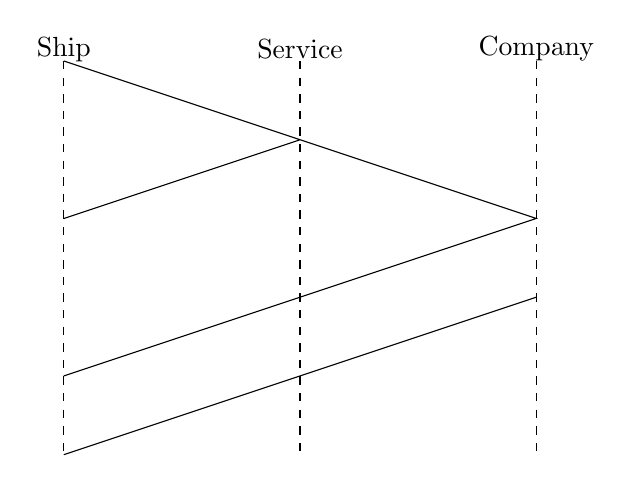
\begin{tikzpicture}
		% timelines
		\draw	[dashed]	(0,5)	--	(0,0)
				[dashed]	(3,5)	--	(3,0)
				[dashed]	(6,5)	--	(6,0);
		% labels
		\draw	(0,5.15)	node	{Ship}
				(3,5.15)	node	{Service}
				(6,5.15)	node	{Company};
		% interaction lines
		\draw	(0,5)	--	(3,4)	--	(0,3)				% API call (request/response)
				(3,4)	--	(6,3)	--	(3,2)	--	(0,1)	% Service requests/recieves data from company/data center
				(6,2)	--	(3,1)	--	(0,0);				% Additional line
	\end{tikzpicture}
	\caption{Rough draft of a model example, where a ship requests something from a service (could be a weather update)}
	\label{fig:modelExProtocol}
\end{figure}
\begin{figure}
	\centering
	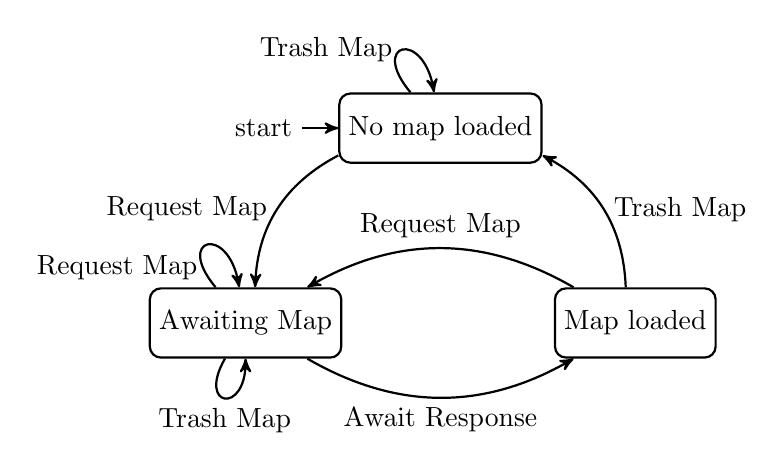
\begin{tikzpicture}[->,>=stealth', node distance=3.5 cm, thick]
		\tikzstyle{every state}=[draw=black,rectangle,rounded corners]

		\node[state, initial]	(A)	[]					{No map loaded};
		\node[state]			(B)	[below left of=A]	{Awaiting Map};
		\node[state]			(C)	[below right of=A]	{Map loaded};

		\path	(A)	edge[bend right,left]									node{Request Map}	(B)
					edge[loop above,left,		out=130,in=100,	looseness=7]node{Trash Map}		(A)
				(B)	edge[loop above,below left,	out=130,in=100, looseness=7]node{Request Map}	(B)
					edge[loop below,below,		out=240,in=270, looseness=7]node{Trash Map}		(B)
					edge[bend right,below]									node{Await Response}(C)
				(C)	edge[bend right,above]									node{Request Map}	(B)
					edge[bend right,right]									node{Trash Map}		(A);
	\end{tikzpicture}
	\caption{Final state machine, describing the \ttt{Ship} entity in Figure \ref{tab:fsmEx}.}
	\label{fig:fsmExShip}
\end{figure}

\begin{figure}
	\centering
	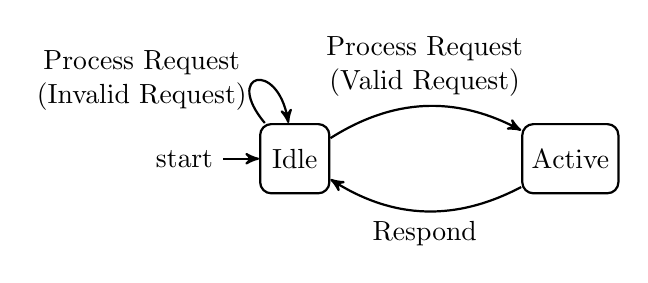
\begin{tikzpicture}[->,>=stealth', node distance=3.5 cm, thick]
		\tikzstyle{every state}=[draw=black,rectangle,rounded corners]

		\node[state, initial]	(A)	[]				{Idle};
		\node[state]			(B)	[right of=A]	{Active};

		\path	(A)	edge[loop above,left,	align=center,	out=130,in=100,	looseness=7]	node{Process Request\\(Invalid Request)}(A)
					edge[bend left,	above,	align=center]									node{Process Request\\(Valid Request)}	(B)
				(B)	edge[bend left,	below]													node{Respond}							(A);
	\end{tikzpicture}
	\caption{Final state machine, describing the \ttt{Service} entity in Figure \ref{tab:fsmEx}.}
	\label{fig:modelExFsm}
\end{figure}

% i XML'en:
%	lav et felt, der hedder entitet
%		definer relation, rolle, etc
%	definer videre på roller, hvad vil de have fra hinanden? Hvad konstituerer en request (på f.esk et kort), skal man bruge adgangskode, hvad sker der hvis den er forkert?


% definér en protokol
% byg på eksisterende entiteter
% 
% vejrudsigt-service
% fra vejrservicens perspektiv:
% et skib anmoder om oplysninger, hvilken informationer skal skibet videregive for at blive tildelt oplysninger
% 
% meget lavpraktisk model:
% tre foruddefinerede modeller, der snakker med hinanden. Simulér en interaktion mellem dem - hvordan skifter de forskellige tilstand når de interagerer?
% hvilke reaktioner kommer der på aktioner?
% opfører en entitet sig rigtigt i forhold til en anden entitet når de interagerer på en bestemt måde?

\section{Model-Based testing of MCP} % Hvad kan man teste med dette?
%TODO

\section{Summary: advantages and disadvantages} 

Issues will inevitably present themselves with a project such as this, however the scope and nature of these issues will vary with each approach possible. As different approaches offer tailored advantages to circumvent correlating unique concerns, another set of unique concerns will necessarily present themselves. In this section I will sum up the approaches presented throughout Chapter \ref{chp:Analysis}, along with their corresponding arising advantages and disadvantages.
\begin{description}
	\item[Manual model-creation]\ \\
	\tbf{Advantages}
	\begin{itemize}
		\item a
		\item b
		\item c
	\end{itemize}
	\tbf{Disadvantages}
	\begin{itemize}
		\item d
		\item e
	\end{itemize}
	\item[Manual model-creation]\ \\
	\tbf{Advantages}
	\begin{itemize}
		\item f
		\item g
		\item h
	\end{itemize}
	\tbf{Disadvantages}
	\begin{itemize}
		\item i
		\item j
		\item k
	\end{itemize}

\end{description}

%Problematikker: F.eks at folk, der lægger software op ikke nødvendigvis selv kan lave modellerne/forstå at give argumenterne, der skal bruges til at generere modeller automatisk
% Diskuter problematikken om at man gerne vil lave tekniske ting, der skal bruges af ikke-tekniske mennesker
%TODO

\displayCounterChp
%%%%%%%%%%%%%%%%%%%%%%%%%%%%%%%%%%%%%%%%%%%%%%%%%%%%%%%%%%%%%%%%%%%%%%%%%%%%%%%
%%% Work                                                                    %%%
%%%%%%%%%%%%%%%%%%%%%%%%%%%%%%%%%%%%%%%%%%%%%%%%%%%%%%%%%%%%%%%%%%%%%%%%%%%%%%%

\chapter{Work/Design}

%What data is available now
\section{Parser Grammars}

\subsection{ServiceSpecificationScema}
\subsection{ServiceDesignSchema}
\subsection{ServiceInstanceSchema}
\subsection{General Grammar}

% Hvordan ville JEG designe en specifikation
% What data WILL be available after?

\section{Implementation in the MCP}

% Evt. lav en specifikationsXML selv.

\section{Technical Implementation}
\subsection{Executing Instructions}

\section{Testing}

\section{Experiments}
\displayCounterChp

%%%%%%%%%%%%%%%%%%%%%%%%%%%%%%%%%%%%%%%%%%%%%%%%%%%%%%%%%%%%%%%%%%%%%%%%%%%%%%%
%%% Experiments and Results                                                 %%%
%%%%%%%%%%%%%%%%%%%%%%%%%%%%%%%%%%%%%%%%%%%%%%%%%%%%%%%%%%%%%%%%%%%%%%%%%%%%%%%

\chapter{Results}



\begin{figure}
	\centering
	\begin{lstlisting}[keywordstyle={}]
Term =
    {entities,
        [{ent,
             [{type,"ship"},
              {name,"Ship"},
              {relations,[{relation,"Service"}]},
              {dependencies,
                  [{dependency,[{to,"Service"},{constraint,"fun psswd"}]},
                   {dependency,[{to,"Service"},{constraint,"fun user"}]}]},
              {information,[]},
              {requests,
                  [{request,
                       [{to,"Service"},
                        {data,"map"},
                        {answers,[{answer,"anton"},{answer,"1234"}]}]}]}]},
         {ent,
             [{type,"service"},
              {name,"Service"},
              {relations,[{relation,"Ship"},{relation,"Company"}]},
              {dependencies,[]},
              {information,[]},
              {requests,[]}]},
         {ent,
             [{type,"company"},
              {name,"Company"},
              {relations,[{relation,"Service"}]},
              {dependencies,[]},
              {information,[{info,"map"}]},
              {requests,[]}]}]}
	\end{lstlisting}
	\caption{Erlang term, resulting of parsing the file \ttt{protocol.xml} with \ttt{main:parse('xml/protocol.xml')}}
	\label{fig:protocolParsed}
\end{figure}


\begin{figure}
	\centering
	\begin{lstlisting}[keywordstyle={}]
[{company,[{<0.79.0>,[]}],<0.78.0>,["map"]},
 {service,[{<0.78.0>,[]},{<0.80.0>,[]}],<0.79.0>,[]},
 {ship,[{<0.79.0>,
         [#Fun<aux.1.111753582>,#Fun<aux.0.111753582>]}],
       <0.80.0>,
       ["map"]}]
	\end{lstlisting}
	\caption{Maritime model, resulting of interpreting the file \ttt{protocol.xml} with \ttt{main:parse\_and\_interpret('xml/protocol.xml')}}
	\label{fig:protocolParsedInterpreted}
\end{figure}
\displayCounterChp

%%%%%%%%%%%%%%%%%%%%%%%%%%%%%%%%%%%%%%%%%%%%%%%%%%%%%%%%%%%%%%%%%%%%%%%%%%%%%%%
%%% Discussion                                                              %%%
%%%%%%%%%%%%%%%%%%%%%%%%%%%%%%%%%%%%%%%%%%%%%%%%%%%%%%%%%%%%%%%%%%%%%%%%%%%%%%%

\chapter{Discussion}
Following the successful development of the solution, described in the preceding chapters, arises problem statements dealing with integration into the MCP, use, future use and the balancing of the compromise that is choosing which model generator to utilize. The following chapter will deal with these topics. Section \ref{sec:Launch and Integration into the MCP} will describe potential approaches to initial integration, while Section \ref{sec:Future Use} will subsequent future use, both practical and technical, following the inevitable need for further development. Section \ref{sec:Manual versus Automatic Model Generation}, will contain an assessment of which model generating functionality is most likely to be widely used, going forth. Eventually, Section \ref{sec:Results Related to Use} will provide a recap of the results, obtained in Chapter \ref{chp:Results}, in relation to what is described in sections \ref{sec:Launch and Integration into the MCP} through \ref{sec:Results Related to Use}.

\section{Launch and Integration into the MCP}
For the solution, described throughout this thesis to be integrated, various changes need to be made with regards to the infrastructure of the Maritime Connectivity Platform. The first, and most obvious, change that should be implemented is the technical implementation of the new functionality. Next comes the need for educating the user-group, as these will have no preceding knowhow as to make the system work in accordance with their needs. This will be necessary, whether use of manual or automatic model generating is utilized.

A soft launch strategy should be used, when inaugurating the functionality, as described in a blog-post on LiveChatInc~\cite{hardoSoft}. Launching the solution gradually will let the user-base to get acquainted with its use, while simultaneously allowing for necessary feedback towards the functionality. This will, in turn, decrease the risk of the project succumbing to any of the launch failures, as described in an article on Harvard Business Review~\cite{hbr}, all of which are often connected with a hard product launch.
\section{Future Use}
Post-launch of the model-building component is a continuous development process. User-submitted feedback should be regularly implemented in order to ensure optimal user friendliness, and intuitiveness. Furthermore as, the functionality, described in Chapter \ref{chp:Work/Design} is only the initial functionality, and ideally, as described in Section \ref{ssec:Expanding Automatic Model Functionality} below, future development is deeply rooted in the project.

\subsection{Expanding Automatic Model Functionality}
Embedded in the nature of the project is the need for future expansion of functionality, following increased demands from maritime service providers. The modularity that the solution has been implemented with will aid in this, as it allows for less complicated employment hereof. As described in Section \ref{sec:Technical Implementation}, the complete solution has been divided into three fields, and thus these are the areas, where further implementation is needed if additional model functionality is desired.
\begin{itemize}
  \item \ttt{mmods.erl}
    The primary functionality will need to be implemented here. This entails the main API call to the finite state machine, along with its following desired result and side effects. Altering the implementation of this file will subsequently alter the manual as well as the automatic model generator.
  \item \ttt{parser.erl}
    This file will \tit{not} need any adjustments in order to handle new functionality.
  \item \ttt{interpreter.erl}
    This file will need to be altered in order to handle additional information, picked up by the parser. In the case that support for model functionality has been implemented in \ttt{mmods.erl}, but not \ttt{interpreter.erl}, said functionality will not be included in the resulting model, and no error or exception will be raised. This is true, even if the additional design information is included in the xml-specification file.
\end{itemize}

\subsection{Expanding Manual Model Functionality}
As explained in Section \ref{ssec:The parser and interpreter modules} the manual component, provides all core functionality of the automatic component. The fact that this module is underdeveloped, in comparison to its automatic counterpart does in no way rule it out for future use, as having only the core functionality encapsulated in a module, providing an all-inclusive API allows for virtually limitless further development. The automatic component is \tit{one} example out of a virtually endless pool of additional functionality, based on the functionality, provided in the manual component. Expanding upon this, will be confined to future work, as potential solutions can scope to an extent similar to this project.

\section{Manual versus Automatic Model Generation}
A fundamental obstacle throughout the project is the learning curves, described in Figures \ref{fig:serialMBT} and \ref{fig:sequenceMBT}, along with their corresponding sections. This obstacle is present in both scenarios, however, the learning curve is significantly steeper, using sequential\footnote{Manual} model based testing/model generating. A soft launch and extensive user-guide, as described in Section \ref{sec:Launch and Integration into the MCP} will reduce the effects of the learning curve for both development techniques, however not to the extend that this is completely negated.

Automatic model generation is, however, both the most user-friendly method and the one most suited for a visual builder interface. A visual builder interface could be in a style, similar to the Eclipse Visual Editor, Vex~\cite{vex} for XML. Such an XML-builder should be implemented to always show the user which options are available to add to the xml and subsequent model, which would in turn ease work flow, placed on all other aspects of the solution.

\section{Results Related to Use}
Taking the findings of Chapter \ref{chp:Results} into consideration, when comparing the usefulness of the two methods, one model-generating technique clearly stands out, as being the most useful. Recognizing that automatic model-generation will provide more immediate user-friendliness, more scalability and, according to Section \ref{ssec:Model Equivalence}, functionality equivalent to that of manual model-generation.

Manual model generation, in it's basic state, as described in Section \ref{ssec:Expanding Manual Model Functionality} allows for limitless new functionality, and, as proven by the implementation of the automatic component, said new functionality does not necessarily need to be manual.

In conclusion, both components add relevant functionality to the MCP, and while automatic model generating provides the more present, needed, service, the manual component provides a broad foundation for development of new ideas.



\displayCounterChp

%%%%%%%%%%%%%%%%%%%%%%%%%%%%%%%%%%%%%%%%%%%%%%%%%%%%%%%%%%%%%%%%%%%%%%%%%%%%%%%
%%% Conclusion                                                              %%%
%%%%%%%%%%%%%%%%%%%%%%%%%%%%%%%%%%%%%%%%%%%%%%%%%%%%%%%%%%%%%%%%%%%%%%%%%%%%%%%

\chapter{Conclusion}

\section{Conclusions}

\section{Future work}

\section{Summary}
\displayCounterChp

%%%%%%%%%%%%%%%%%%%%%%%%%%%%%%%%%%%%%%%%%%%%%%%%%%%%%%%%%%%%%%%%%%%%%%%%%%%%%%%
%%% BIBLIOGRAPHY                                                            %%%
%%%%%%%%%%%%%%%%%%%%%%%%%%%%%%%%%%%%%%%%%%%%%%%%%%%%%%%%%%%%%%%%%%%%%%%%%%%%%%%

\cleardoublepage
\renewcommand{\sc}[1]{\textsc{#1}}
\bibliographystyle{acm}
\bibliography{bibliography}

%%%%%%%%%%%%%%%%%%%%%%%%%%%%%%%%%%%%%%%%%%%%%%%%%%%%%%%%%%%%%%%%%%%%%%%%%%%%%%%
%%% RESEARCH PAPERS                                                         %%%
%%%%%%%%%%%%%%%%%%%%%%%%%%%%%%%%%%%%%%%%%%%%%%%%%%%%%%%%%%%%%%%%%%%%%%%%%%%%%%%

\begin{thebibliography}{9}
	\bibitem{mcp}
		Maritime Connectivity Platform,
		\url{https://maritimeconnectivity.net/}
	\bibitem{quickcheck}
		QuviQ,
		\url{http://www.quviq.com/}
	\bibitem{efficienSea2}
		EfficienSea2's website,
		\url{https://efficiensea2.org/solution/maritime-connectivity-platform/}
	\bibitem{realWorldHaskell11}
		Real World Haskell,
		Bryan O'Sullivan, Don Stewart, and John Goerzen,
		Chapter 11,
		\url{http://book.realworldhaskell.org/read/testing-and-quality-assurance.html}
	\bibitem{nlp}
		Natural Language Processing,
		Elizabeth D. Liddy,
		Syracuse University,
		\url{liddy@syr.edu}
		\url{http://surface.syr.edu/cgi/viewcontent.cgi?article=1019&context=cnlp}
	\bibitem{memoization}
		Monadic Memoization towards Correctness-Preserving Reduction of Search
		Richard Frost
		School of Computer Science, University of Windsor
		Ontario, Canada
		\url{richard@uwindsor.ca}
		\url{http://richard.myweb.cs.uwindsor.ca/PUBLICATIONS/AI_03.pdf}
	\bibitem{xmerl}
		xmerl reference manual,
		\url{http://erlang.org/documentation/doc-5.4/pdf/xmerl-1.0.pdf}
	\bibitem{xmerlEx}
		Starting to play with xmerl,
		Arif Ishaq,
		\url{https://arifishaq.wordpress.com/2014/11/25/starting-to-play-with-xmerl/}
\end{thebibliography}


\appendix

\chapter{Appendix}

\section{token}
\begin{figure}[h]
  \begin{lstlisting}
token(String) ->
  case String of
    % atoms
    "ship"    -> ship;
    "service" -> service;
    "company" -> company;
    % functions
    "fun psswd"   -> fun aux:psswd/1;
    "fun user"    -> fun aux:user/1;
    "fun trivial" -> fun aux:trivial/1;
    _             -> error
  end.
  \end{lstlisting}
  \caption{The \ttt{token/1}-function in the \ttt{aux}-file.}
\end{figure}
\newpage
\section{ServiceSpecificationSchema}
\begin{figure}[h]
	\centering
	\begin{lstlisting}[keywordstyle={},breaklines=true]
ServiceSpecificationSchema ::= specifications

specifications ::= spec specifications
     | $\e$
     
spec ::= name
     | status
     | id
     | version
     | description
     | keywords
     | isSpatialExclusive
     | authorInfos
     | requirements
     | serviceDataModel
     | serviceInterfaces
     
authorInfos ::= authorInfo authorInfos
     | $\e$

authorInfo ::= aSpec authorInfo
     | $\e$

aSpec ::= id
     | name
     | description
     | contactInfo

requirements ::= requirement requirements
     | $\e$
     \end{lstlisting}
     \caption{Full parser grammar of Service Specification Schema. (1 of 2)}
     \label{fig:sSpecFull1}
\end{figure}
\newpage
\begin{figure}[h!]
     \centering
     \begin{lstlisting}[keywordstyle={}]

requirement ::= rSpec requirement
     | $\e$

rSpec ::= id
     | name
     | text

serviceDataModel ::= definitionAsXSD

definitionAsXSD ::= $\e$

serviceInterfaces ::= serviceInterface serviceInterfaces
     | $\e$

serviceInterface ::= siSpec serviceInterface
     | $\e$

siSpec ::= name
     | description
     | dataExchangePattern
     | operations

operations ::= operation operations
     | $\e$

operation ::= oSpec operation
     | $\e$

oSpec ::= name
     | description
     | returnValueType
     | parameterTypes

returnValueType ::= typeReference


parameterTypes ::= parameterType parameterTypes
     | $\e$

parameterType ::= ptSpec parameterType
     | $\e$

ptSpec ::= typeReference
	\end{lstlisting}
	\caption{Full parser grammar of Service Specification Schema. (2 of 2)}
	\label{fig:sSpecFull2}
\end{figure}
\section{E2 - NW-NM Service Specification}
\lstinputlisting{figures/E2.xml}

\displayCounters
% Each paper is defined as a new section of an appendix chapter. This means that they automatically are added to TOC and it is possible to refer to them.

% Updates section names to remove . (e.g. a section is named A1 instead of A.1)
\renewcommand{\thesection}{\thechapter\arabic{section}}

\end{document}

% Til vejledning?
%
% - Baggrund skal være længere (40/50 sider i alt er fino)
%   - beskriv teknikker (property/model-based testing)
%
% - lav i første omgang en model på baggrund af min specifikation (manuel)
% - lav i anden omgang en model på baggrund af min specifikation (automatisk)
